\documentclass[12pt]{article}

\usepackage{float}
\usepackage{amsmath}
\usepackage{amsfonts}
\usepackage{tikz}
\usepackage{pgfplots}

\begin{document}
\title{AP Physics C: Newton's 3\textsuperscript{rd} Law}
\author{Raja Williams}
\date{November 2023}
\maketitle

\section{Objective}
The Newton's 3\textsuperscript{rd} Law lab includes experimentally calculating
the $\mu_k$ of the interaction between a friction block connected to the cart in
a half-Atwood machine, and the track of the half-Atwood machine.

\section{Procedure}
\begin{enumerate}
    \item First, before preparing the half-Atwood machine, measure the mass of
        the cart and the friction block.
    \item Set up the experiment as shown in Figure \ref{fig:step2}.
    \begin{figure}[h]
        \centering
        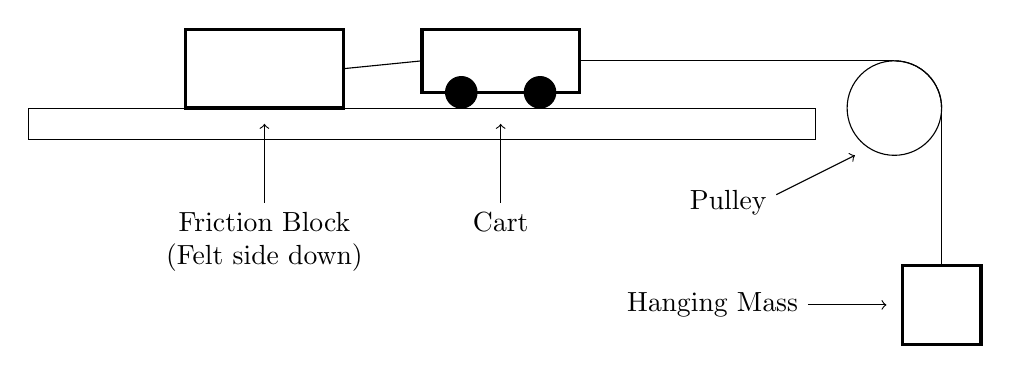
\begin{tikzpicture}
            \draw[very thick] (2,0.2) rectangle (0,1);
            \draw[fill=black] (0.5,0.2) circle [radius=0.2];
            \draw[fill=black] (1.5,0.2) circle [radius=0.2];
            \draw[very thick] (-1,0) rectangle (-3,1);
            \draw (-1,0.5) -- (0,0.6);
            \draw (6,0) circle [radius=0.6];
            \draw (6.6,0) arc (0:90:0.6);
            \draw (2,0.6) -- (6,0.6);
            \draw (6.6,0) -- (6.6,-2);
            \draw[very thick] (6.1,-2) rectangle (7.1,-3);
            \draw (-5,0) rectangle (5,-0.4);
            \draw[->] (1,-1.2) -- (1,-0.2);
            \draw (1,-1.2) node[anchor=north] {Cart};
            \draw[->] (4.5,-1.1) -- (5.5,-0.6);
            \draw (4.5,-1.2) node[anchor=east] {Pulley};
            \draw[->] (4.9,-2.5) -- (5.9,-2.5);
            \draw (4.9,-2.5) node[anchor=east] {Hanging Mass};
            \draw[->] (-2,-1.2) -- (-2,-0.2);
            \draw (-2,-1.2) node[anchor=north,align=center] {Friction Block\\(Felt side down)};
        \end{tikzpicture}
        \caption{Diagram of Step 2 experimental setup.}
        \label{fig:step2}
    \end{figure}
    \item Start data collection on the sensor cart.
    \item Let go of the sensor cart.
    \item Stop data collection when cart collides with pulley.
    \item Determine the acceleration of the cart from the data collected.
    \item Repeat from Step 3, adding mass to the system via adding masses to the
        top of the cart. We chose three trials with extra masses of 0 grams, 200
        grams, and 250 grams.
\end{enumerate}

\section{Observations and Data}

From Step 1, we found that the cart was 0.282 kilograms. As well, we found that
the friction block was 0.331 kilograms.

From Steps 3-7, we captured three data points, shown in Figure \ref{fig:table}.

\begin{figure}[H]
    \centering
    \begin{tabular}{| r | l | l |}
        \hline
        Trial & $m$ (g) & $a$ (m/s\textsuperscript{2}) \\ \hline
        1 & 0 & 0.418 \\
        2 & 200 & 0.305 \\
        3 & 250 & 0.275 \\
        \hline
    \end{tabular}
    \caption{Table of the data captured from Steps 3-7.}
    \label{fig:table}
\end{figure}

\section{Analysis}

Using data collected from Step 1, the mass of the entire system, which includes
the mass, the cart, and the block, would be 0.663 kg. If we shift the data
points acquired from Steps 3-7, we can find a correlation between the mass of
the system and the final acceleration of the system. These new data points can
be seen in Figure \ref{fig:correlation}.

\begin{figure}[h]
    \centering
    \begin{tabular}{| r | l | l |}
        \hline
        Trial & $m$ (kg) & $a$ (m/s\textsuperscript{2}) \\ \hline
        1 & 0.663 & 0.418 \\
        2 & 0.863 & 0.305 \\
        3 & 0.913 & 0.275 \\
        \hline
    \end{tabular}
    \caption{Table of the modified data derived from Steps 3-7.}
    \label{fig:correlation}
\end{figure}

The line of best fit for these new data points in Figure \ref{fig:correlation}
is $a(m) = -0.57m + 0.796$. Since, for the system as a whole, $\Sigma F = ma = F_g
- F_{f_k}$, we can solve for $F_{f_k}$. Using the line of best fit for the
acceleration as a function of system mass, we can calculate $F_{f_k}$ as a
function of system mass by doing:

\begin{align}
    \begin{split}
        F_g &= 0.050 \text{ kg} \cdot 9.8 \text{ m/s\textsuperscript{2}} \\
        F_g &= 0.49 \text{ N} \\
        m \cdot a(m) &= F_g - F_{f_k} \\
        m \cdot a(m) &= 0.49 \text{ N} - F_{f_k} \\
        -m \cdot a(m) + 0.49 \text{ N} &= F_{f_k}
    \end{split}
\end{align}

Now, substituting in $a(m)$:

\begin{align}
    \begin{split}
        -m \cdot a(m) + 0.49 \text{ N} &= F_{f_k} \\
        -m(-0.57m + 0.796) + 0.49 \text{ N} &= F_{f_k} \\
        0.57m^2 - 0.796m + 0.49 \text{ N} &= F_{f_k}
    \end{split}
\end{align}

This means that $F_{f_k}$ is a function of the mass of the entire system. With
the $F_{f_k}$, we can now find $\mu_k$. Since $F_{f_k} = \mu_k \cdot F_N$,
utilizing the mass of the block measured earlier, we can finally extract
$\mu_k$.

\begin{align}
    \begin{split}
        F_N &= 0.331 \text{ kg} \cdot 9.8 \text{ m/s\textsuperscript{2}} \\
        F_N &= 3.244 \text{ N} \\
        F_{f_k} &= \mu_k \cdot F_N \\
        0.57m^2 - 0.796m + 0.49 \text{ N} &= \mu_k \cdot 3.244 \text{ N} \\
        \frac{0.57m^2 - 0.796m + 0.49 \text{ N}}{3.244 \text{ N}} &= \mu_k
    \end{split}
\end{align}

A plot of the modified $a$ data points, $a(m)$, $F_{f_k}$, and $\mu_k$ is visible in Figure
\ref{fig:compilation}.

\begin{figure}[H]
    \centering
    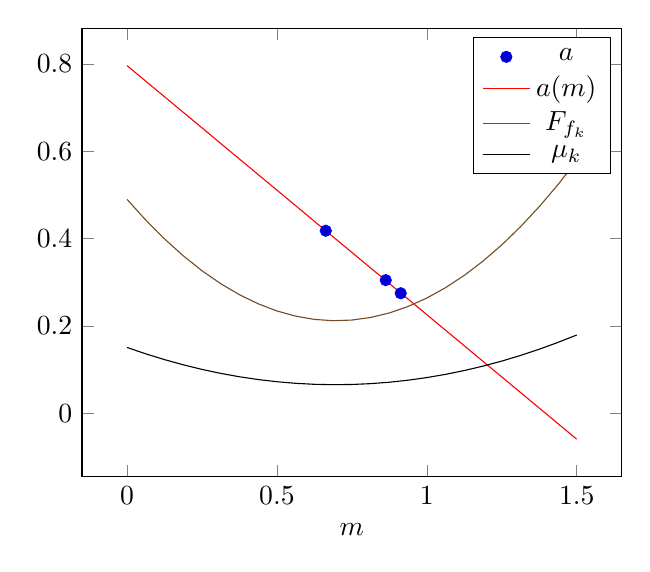
\begin{tikzpicture}
        \begin{axis}[xlabel=$m$, domain=0:1.5]
            \addplot+[only marks] coordinates {
                (0.663, 0.418)
                (0.863, 0.305)
                (0.913, 0.275)
            };
            \addplot+[no markers] {-0.57*x+0.796};
            \addplot+[no markers] {0.57*x^2-0.796*x+0.49};
            \addplot+[no markers] {0.176*x^2-0.245*x+0.151};
            \legend{$a$, $a(m)$,$F_{f_k}$,$\mu_k$}
        \end{axis}
    \end{tikzpicture}
    \caption{Plot of $a$, $a(m)$, $F_{f_k}$, and $\mu_k$ as functions of $m$.}
    \label{fig:compilation}
\end{figure}

We then averaged the $\mu_k$ at the three $m$ data points, and got a final
answer of $\overline{\mu_k} = 0.090$.

\section{Conclusion}
The expected value for the $\mu_k$ was 0.304, which means a percent error for
our calculated value of about 70.55\%. The likely reason for this anomaly is
likely that, for one, the scale provided is inconsistent and not fully accurate,
leading some of our mass values to be off. As well, we did not ensure data
reliability by doing multiple trials at one mass. The tiny sample size of the
final data does imply that there could be unreliability underlying the data.

\end{document}
